\documentclass{tufte-handout}
\usepackage[utf8]{inputenc}
\usepackage[T1]{fontenc}
\usepackage{tikz}
\usepackage{listings}

\title{Head First Java: Chapter 11 Notes}
\lstset{language=java, basicstyle={\small\ttfamily}, breaklines=false}

\begin{document}

    \maketitle

    \section*{Throwing and Catching Exceptions}
    In Java, exceptions handling involves declaring (\emph{throwing}) anticipated possible exceptions in methods, and acknowledging plausible exceptions in method calls (\emph{catching}). Practically all properly developed Java API's classes and methods throws exceptions, and they can be seen in their documentation online. For example, the documentation for \texttt{javax.sound.midi.Sequencer.getSequencer()} throws the \texttt{MidiUnavailableException}. Because this particular exception was \emph{thrown} in the method declaration and description, when calling it elsewhere it must be caught via the \texttt{\textbf{try...catch...finally}} block. For example, in order to use the \texttt{getSequencer()} method described just now:

    \begin{lstlisting}
import javax.sound.midi.*;

public class MusicTest1 {
    public void play() {
        try {
            Sequencer sequencer = MidiSystem.getSequencer();
            System.out.println(``Successfully got a sequencer.'');
        } catch(MidiUnavailableExeption ex) {
            System.out.println(``Fail to get sequencer.'');
            ex.printStackTrace();
        }
    }
}
    \end{lstlisting}

    This is similar to Python try/except blacks except in Java it is \emph{mandatory}, if a method throws a (or more than one) exception(s), code that calls that method \textbf{must} use the try/catch block to anticipate it/them. In the above example, the \texttt{play()} method will run the \texttt{Sequencer sequencer = MidiSystem.getSequencer();} line of code, if it success, it will run the remaining code in the \texttt{try} block. If a \texttt{MidiUnavailableExeption} occur, the compiler will store the error in the exception object \texttt{ex}, and skip the remaining code in the \texttt{try} block, and run the code in the \texttt{catch} block instead. Code in the \texttt{catch} block is not ran unless the declared exception occurred. Because of this, the code within the \texttt{catch} block is usually to the last chance to recover from the exception to ensure the program will continue to run, otherwise this is an opportunity to regularly exit from the program, rather than crashing. Using the \texttt{printStackTrace()} or other diagnostic method, the user can then proceed to investigate what went wrong.

    To throw exceptions in a method, it must be declared first. For example:

    \begin{lstlisting}
public void takeRisk() throws BadException {
    if (exceptionOccurs) {
    throw new BadException();
    }
}

public void tryingRisks() {
    try {
        anObject.takeRisk();
    } catch(BadException ex) {
        System.out.println(``Bad exception occurred.'')
    }
}
    \end{lstlisting}

    Note that in the above example, \texttt{BadException} is not a real and defined \texttt{Exception} subclass object, but user-defined exceptions can be defined just like any other objects. The reasoning of the above code listing is that, while writing \texttt{takeRisk()} as a method, the user anticipated a specific exception \texttt{BadException}, which must be declared at the method declaration with keyword \texttt{throws}. Multiple exceptions can be declared here, separated by commas. Then, within the body of the method code, the exception can be thrown by using the \texttt{throw} keyword by initializing a object of the exception (also using the \texttt{new} keyword.) Once the exception is declared and the initialization of the exception is properly coded in the method, whenever the method is called, the exception must be caught via a try/caught block. If multiple exceptions were thrown, they must all be caught.

    \section*{Exception Categories and Hierarchy}
    Exceptions are handled like objects in Java. All declarable exceptions are a subclass of class \texttt{Exception} (which like all objects is a subclass of \texttt{Object}). All subclasses of \texttt{Exception} are checked during compilation by the Java compiler, except for the subclass \texttt{RuntimeException} and its own subclasses. By definition, \emph{runtime exceptions} occur only at runtime, and usually due to either faulty code logic or user input. Runtime exceptions should not be caught by try/catch blocks but rather should be avoided through thorough testing and proper coding. 

    \section*{Flow Control in \texttt{Try/Catch} Blocks}
    As mentioned above, code in \texttt{try} and \texttt{catch} blocks are in an either/or situation. Consider the following code listing:

    \begin{lstlisting}
try {
    Foo f = x.doRiskyThing();
    int b = f.getNum();
} catch (SomeException ex) {
    System.out.println(``Failed.'')
} finally {
    System.out.println(``Exiting...'')
}
System.exit(0);
    \end{lstlisting}

    There are two lines of code within the \texttt{try} block, how many of them run depends on if and when \texttt{SomeException} was thrown. If no exception was thrown, all code within the \texttt{try} block will run, then all code within the \texttt{catch} block will be skipped. If \texttt{SomeException} does get thrown, one or two lines of the code may be ran within the \texttt{try} block, depending when the exception was thrown. Regardless, once the exception was thrown, all code within the \texttt{try} block is skipped, and the code within the \texttt{catch} block is ran. The \texttt{finally} block is optional, but it is always ran regardless when all possible flow within the try/catch block. Code that exist outside of the try/catch(/finally) block only runs when all code within the block(s) are ran according the the flow described above (note that it is possible for the flow of the code within the block to lead elsewhere other than the next line if code outside of the block, \textit{e.g.} via \texttt{return} or exiting the program within the \texttt{catch} block; if that occurs, the code outside the try/catch block might not run, but code within the \texttt{finally} block \emph{will} run regardless.)

    \section*{Exceptions and Polymorphism}
    Because exceptions in Java are objects, all polymorphism concepts and behavior applies. If an exception is thrown, it can be caught by a superclass of the exception, but not the other way around. Because all exceptions are subclasses of \texttt{Exception}, theoretically \texttt{Exception} can catch all possible exceptions, but this is bad coding practices as it will lead to ambiguity on what exact exception has occur, and hence recovery would be difficult. If multiple exceptions are thrown, and they are of from the same inheritance tree but of a different hierarchal level, when coding the multiple \texttt{catch} blocks, they must be in the order from bottom subclass towards the superclass. The reason is if they are out of order, the exception that exist higher on the inheritance tree will catch all thrown exceptions that includes itself and its subclass, which leaves the \texttt{catch} block code intended to catch exceptions at a lower inheritance position meaningless. 

    \section*{Exception Ducking}
    When exceptions are thrown, they have to be caught eventually. However, it is possible to pass exceptions along a chain of method calls, which catches the exception at this end without intervention in the intermittent method calls. Consider:

    \begin{lstlisting}
public class Washer {
    Laundry laundry = new Laundry();
    public void foo() throws ClothingException {
        laundry.doLaundry();
    }
    public static void main(String[] args) {
        Washer a = new Washer();
        a.foo(); 
    }
}
    \end{lstlisting}

    The above code illustrate a case where the code will compile but at runtime it will run into problems. Assuming that \texttt{doLaundry()} and class \texttt{Laundry} is properly defined and that the method throws a \texttt{ClothingException}, it would appear that there isn't any code written to catch the thrown method due to all the method ducking the thrown exception. The above (assume that the classes \texttt{Laundry}, \texttt{Washer}, and the exception \texttt{ClothingException} are properly defined elsewhere), when ran, can be visualized on the stack as such:

    \begin{center}
        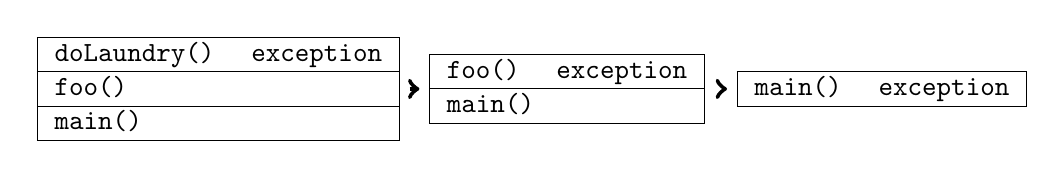
\begin{tikzpicture}
            \node (a) {
                \begin{tabular}{ |l| }
                    \hline \texttt{\textbf{doLaundry()}} \quad \texttt{exception} \\ 
                    \hline \texttt{\textbf{foo()}} \\ 
                    \hline \texttt{\textbf{main()}} \\ 
                    \hline     
                \end{tabular}
            };
            \node[xshift=2cm] (b) at (a.east) {
                \begin{tabular}{ |l| }
                    \hline \texttt{\textbf{foo()}} \quad \texttt{exception} \\ 
                    \hline \texttt{\textbf{main()}} \\  
                    \hline     
                \end{tabular}
            };
            \node (c) at (b.east) {};
            \draw[->,ultra thick](a)--(b);
            \node[xshift=2cm] (d) at (c.east) {
                \begin{tabular}{ |l| }
                    \hline \texttt{\textbf{main()}} \quad \texttt{exception} \\ 
                    \hline    
                \end{tabular}
            };
            \draw[->,ultra thick](c)--(d);
        \end{tikzpicture}
    \end{center}

    This the stack visualization above, \texttt{main()} first appear on the stack, which (aside from initiating a \texttt{Washer} class object and assigning it to reference variable \texttt{a}) runs the method \texttt{foo()}, whose frame is now in scope above the \texttt{main()} frame. Then, \texttt{foo()} calls the method \texttt{doLaundry()}, whose frame is now at the top of the stack. As mentioned earlier, \texttt{doLaundry()} initiates the \texttt{ClothingException} object and throws it (not shown above). As \texttt{doLaundry()} resolves and is popped of the stack, \texttt{ClothingException} is thrown to the method that called it, in this case \texttt{foo()}, whose frame is now in scope. However, as shown above, \texttt{foo()} has no try/catch code block to catch \texttt{ClothingException}, rather, it declares that it throws \texttt{ClothingException} without actually including code to throw a new instance of the exception. In this case, the \texttt{ClothingException} is ``\emph{ducked}'', which means it avoid catching the exception and expects another method call below it on the stack to catch it. The code above was deliberately written to cause a runtime exception, because as \texttt{foo()} is popped off the stack, the exception is thrown further down to \texttt{main()}, which like \texttt{foo()}, also throws \texttt{ClothingException} and has no try/catch block to catch the exception. This is cause runtime exception that shuts down the JVM at run time. Therefore, as many ducks can be used to pass exception down the stack, but it must eventually be caught before it reaches \texttt{main()} to avoid runtime errors.  

\end{document}